%!TEX TS-program = xelatex
\documentclass{schoens-cv}
\usepackage{tikz}
\usetikzlibrary{mindmap,trees}

\begin{document}
\header{paul}{schoenfelder}
       {software developer}
       
% In the aside, each new line forces a line break
\begin{aside}
  \section{where}
    195 5th St E
    APT 3003
    Saint Paul
    MN
    
  \section{online}
    \href{mailto:paulschoenfelder@gmail.com}{paulschoenfelder@gmail.com}
    
    \href{https://github.com/bitwalker}{github.com/bitwalker}
    
  \section{languages}
	{\setlength{\tabcolsep}{0.5em}%
  	\begin{tabular}{ r | c }
    		C\# & \skilled \love
    		JavaScript & \skilled \love
    		CoffeeScript & \skilled \love
  		Ruby & \skilled \love
  		Clojure & \love
  		Go & \love
  		HTML {\bf 5} & \skilled
  		CSS {\bf 3} & \skilled
  		SASS & \skilled \love
    	\end{tabular}}
\end{aside}

\section{interests}

programming languages, design, data mining, artificial intelligence,
craft beer, snowboarding, motorcycles, music, the future

\section{education}

\begin{entrylist}
	\entry
    		{thru 2012}
    		{Completionist {\normalfont many online courses}}
    		{Coursera}
    		{%
    			{\emph{Introduction to Mathematical Thinking}} \\
    			{\emph{Machine Learning}} \\
    			{\emph{Algorithms, Part I}} \\
    			{\emph{Cryptography I}} \\
    			{\emph{A History of the World since 1300}} \\
    			{\emph{Introduction to Astronomy}} \\
    			{\emph{Calculus: Single Variable}}%
    		}
  	\entry
  		{2010-2011}
  		{AAS {\normalfont Avionics Systems Technology}}
  		{Community College of the Air Force}
  		{\emph{Avionics Systems Theory and Maintenance}}
\end{entrylist}

\section{experience}

\begin{entrylist}
	\entry
		{since May}
		{Senior Software Developer}
		{Surge LLC.}
		{Lead developer on three projects. Developed expertise with Adobe InDesign Server and %
		 InDesign Markup Language.}
	\entry
		{2010-2012}
		{Software Developer}
		{ProtoLabs Inc.}
		{Primary developer of numerous projects. Most developers at ProtoLabs fit in to one of two teams, %
		 web or backend - I was the exception, primarily devoted to R\&D applications with focus towards %
		 internal process improvement and reporting/data mining capability.}
	\entry
		{since 2010}
		{Avionics Systems Journeyman}
		{United States Air Force}
		{My second job is with the Air National Guard/USAF out of Madison, WI - where I work as a flightline %
		 avionics technician on Lockheed Martin F-16C/D fighter jets. I'm currently a Senior Airman, working %
		 towards my Staff Sergeant stripes.}
	\entry
		{2008-2010}
		{Software Developer}
		{Business Card Services Inc.}
		{The entirety of my time at BCSI was spent as the primary developer behind a project to port a %
		 legacy manufacturing process written and maintained since the late 80's to a modern, C\# and ASP.NET %
		 driven system, while expanding it's capabilities, and providing some new reporting and data mining %
		 features that the old system could not provide. After the first release of the new software, I left %
		 for training with the United States Air Force.}
	\entry
		{2006-2008}
		{Software Developer}
		{Warner Connect Inc.}
		{I started at WC as a Network Engineer - architecting, implementing and maintaining new network %
		 systems at our clients locations. Within six months however, I had convinced my boss to let me take %
		 over the newly formed Development branch of the company, and begin my professional career in software%
		  development. This was where I first gained exposure to C\#, ASP.NET, Classic ASP, T-SQL, and all of %
		 tools and techniques that come along with them.}
\end{entrylist}

\section{developed skills}

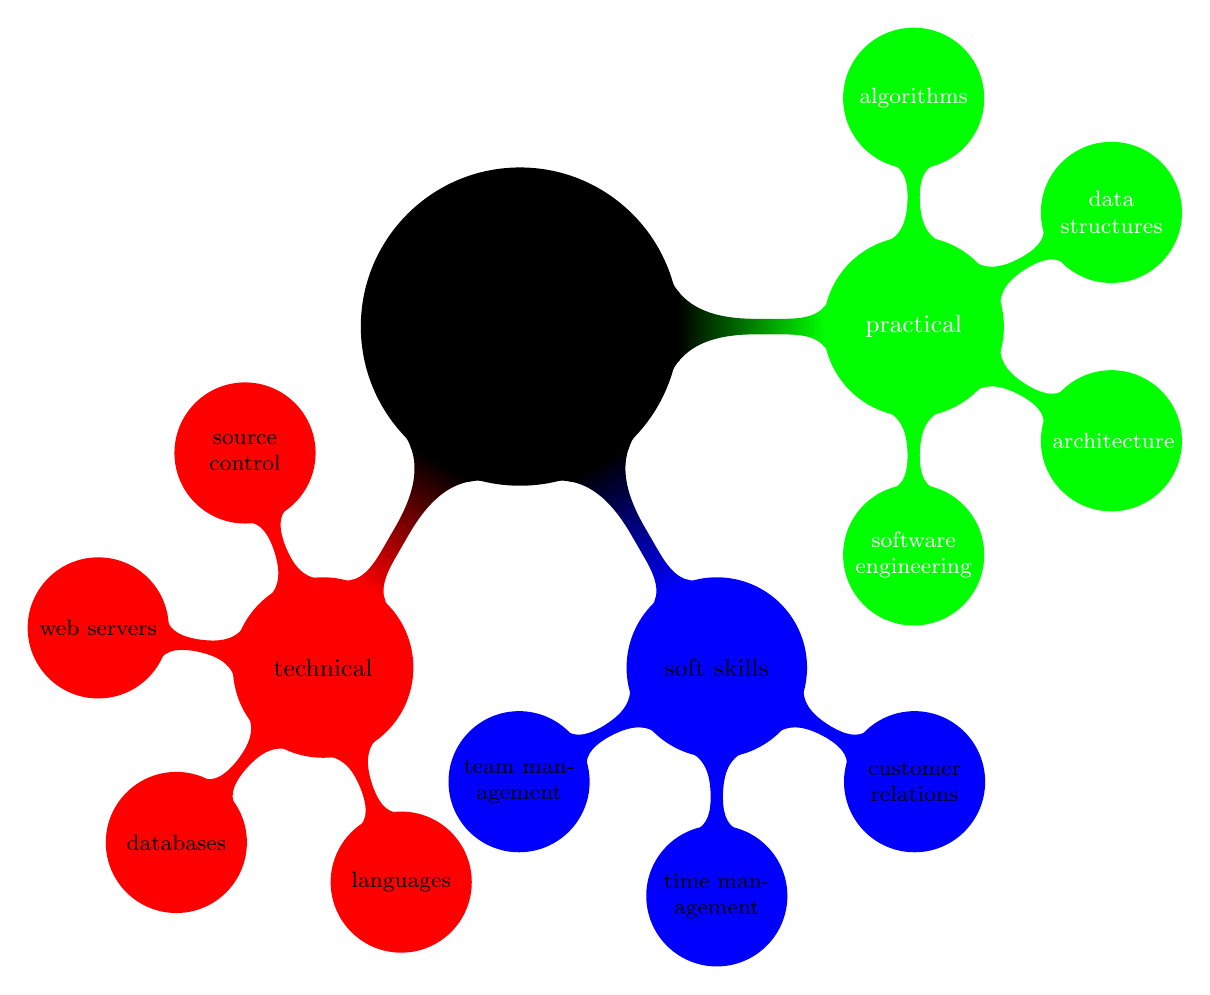
\begin{tikzpicture}
	\path[mindmap,concept color=black]
		node[concept] {Software \\ Development}
		[clockwise from=0]
    		child[concept color=green,text=white] {
      		node[concept] {practical}
      		[clockwise from=90]
      		child { node[concept] {algorithms} }
      		child { node[concept] {data structures} }
      		child { node[concept] {architecture} }
      		child { node[concept] {software engineer\-ing} }
    		}  
    		child[concept color=blue] {
      		node[concept] {soft skills}
      		[clockwise from=-30]
      		child { node[concept] {customer relations} }
      		child { node[concept] {time management} }
      		child { node[concept] {team management} }
    		}
    		child[concept color=red] { 
    			node[concept] {technical}
    			[clockwise from=-70]
    			child { node[concept] {languages} }
    			child { node[concept] {databases} }
    			child { node[concept] {web servers} }
    			child { node[concept] {source control} }
    		};
\end{tikzpicture}

\section{proficiencies}

\begin{entrylist}
	\entry
		{Languages}
		{I could almost speak them...}
		{}
		{%
			\hilite{C\#}, Ruby, Go, Clojure,
			\hilite{JavaScript, CoffeeScript,}
			Powershell, C/C++, \hilite{HTML, CSS, SASS}
		}
	\entry
		{Tools}
		{What is a workman without his tools...}
		{}
		{%
			\hilite{Visual Studio}, Sublime Text, \hilite{Git}, Mercurial,
			Subversion, \hilite{NUnit}, MSpec, Moq, TypeMock, CruiseControl
		}
	\entry
		{Platforms}
		{A strong foundation to build upon...}
		{}
		{%
			\hilite{ASP.NET MVC, Node.js, } Rails,
			Noir, \hilite{Knockout.js}, Underscore.js, Backbone.js, \hilite{jQuery}
		}
\end{entrylist}

       
\end{document}